\chapter{Implémentation et résultats}
Le chapitre précédent a montré que nous avons réussi à modéliser un problème de planification prenant en compte un environnement, une mission et un aéronef dans un langage de contraintes. Nous pouvons donc tester différents outils à notre disposition pour implémenter notre démarche et l'éprouver.

\`A présent nous allons présenter plusieurs solveurs CSP ainsi que ce que nous avons réussi à implémenter et les résultats que nous avons eus. Les solveurs qui nous intéressent doivent être capables de prendre en compte des variables entières et réelles, de plus ils doivent permettre l'écriture de contraintes quadratiques pour réussir à utiliser nos contraintes de stabilité ellipsoïdales.
En premier nous présentons JaCoP, un solveur CSP supportant des variables et contraintes continues, puis CPLEX, un solveur de programmation linéaire et quadratique.

\section{JaCoP}
%\subsection{Les différences entre la modélisation souhaitée et l'implémentation JaCoP}
Nous avons utilisé JaCoP\footnote{\url{http://http://jacop.osolpro.com/}} (Java Constraint Programming solver) pour implémenter et tester la modélisation et la démarche présentée dans le chapitre \ref{chapter:model}. 

JaCoP permet le travail avec des entiers et des réels, par contre chaque calcul mathématique doit être ramené à une succession d'opération élémentaire ($+, \times, -, \div$), néanmoins les comparaisons sont possibles ainsi que quelques fonctions telles que l'opérateur de puissance ou de valeur absolue.

Une différence avec notre modélisation est la distinction des types de variables. Dans JaCoP toutes les variables de fonction (Cf \ref{variableFonction}) sont des variables de décision (Cf \ref{variableDecision}). Même si JaCoP ne permet pas cette distinction, cela ne diminue pas ses capacités à exprimer le problème de planification tel que nous l'avons présenté.

%Nous avons tout de même souhaité tester ce solveur car cela ne semblait pas être un très gros problème pour la suite.

\subsection{Modélisation de l'aéronef}
%\subsubsection{Encodage d'un espace d'état dans JaCoP}
Nous allons présenter la démarche et les algorithmes utilisées pour la traduction d'un espace d'état de façon générale, la même démarche doit évidemment être appliquée aux différents modes de fonctionnement.

Nous rappelons les notations d'un espace d'état linéaire discrétisé :
\begin{equation}
\label{eq:Xk+1}
X_{k+1} = A.X_k + B.U_k
\end{equation}
\begin{equation}
\label{eq:Yk}
Y_k = C.X_k + D.U_k
\end{equation}
Avec $X_k \in \mathbb{R}^{n}$, $Y \in \mathbb{R}^{r}$, $U_k \in \mathbb{R}^{m}$, $A \in \mathbb{R}^{n\times n}$, $B \in \mathbb{R}^{n\times m}$, $C \in \mathbb{R}^{r\times n}$ et $D \in \mathbb{R}^{r\times m}$

Notre but est de réussir à traduire ces équations en contraintes utilisables par JaCoP, ce qui permettra au solveur de "calculer" les états et les sorties du systèmes durant la planification.

Afin de remplir cet objectif, nous avons créé un algorithme (Cf. Alg. \ref{algo:XktoCSP} et \ref{algo:YktoCSP}) qui permet, à partir d'une modélisation par espace d'état, de générer les contraintes JaCoP le représentant. Le problème est que nous sommes obligé de détailler chaque opération (+,-,$\times$,$\div$), et de stocker le résultat de ces opérations dans des variables temporaires. Le principe est donc de décomposer les différents produits matricielles ainsi que les sommes matricielles (Cf éq \ref{eq:espaceEtatExplose}). 

Pour ce qui est de l'équation \ref{eq:Xk+1} :\\
$
\begin{array}{ccccc}
x_{1,k+1} = a_{1,1}.x_{1,k} + a_{1,2}.x_{2,k} + &\dots& + a_{1,n}.x_{n,k} + b_{1,1}.u_{1,k} +&\dots&+ b_{1,m}.u_{m,k} \\ 
x_{2,k+1} = a_{2,1}.x_{1,k} + a_{2,2}.x_{2,k} + &\dots& + a_{2,n}.x_{n,k} + b_{2,1}.u_{1,k} +&\dots&+ b_{2,m}.u_{m,k} \\ 
\vdots&&\vdots&&\vdots\\ 
x_{n,k+1} = a_{n,1}.x_{1,k} + a_{n,2}.x_{2,k} + &\dots& + a_{n,n}.x_{n,k} + b_{n,1}.u_{1,k} +&\dots&+ b_{n,m}.u_{m,k}
\end{array} 
$

Afin de déterminer le nombre de variable temporaire nécessaire, nous devons compter le nombre d'opération à effectuer. Nous avons donc pour chaque ligne : 
\begin{itemize}
	\item[] $n_{addition} = (n-1) + (m-1) + 1$
	\item[] $n_{multiplication} = n + m$
	\item[] $n_{affectation} = 1$
	\end{itemize}
	Ce qui fait un total de $n_{temp1} = (n_{addition} + n_{multiplication} + n_{affectation})\times n$, soit $n_{temp1} = (n + m)\times 2n$.
	Le même principe est à appliquer à l'équation \ref{eq:Yk}, avec cette fois $n_{temp2} = (n + m)\times 2r$.
	
	Dans le but de faciliter l'implémentation des algorithmes suivants, nous introduisons un tableau de variables temporaires nommé $temp$, ce tableau est de taille $n_{temp} = n_{temp1} + n_{temp2}$. On notera donc $temp_i$ la i-ème variable temporaire.
	\begin{algorithm}[H]
		\LinesNumbered
		\Donnees{$<A,B>$ des matrices du système\\$n$ est le nombre d'états ; $m$ est le nombre d'entrées ; $r$ est le nombre de sorties }
		\Pour{i = 1 à n}{
			\Pour{j = 1 à n}{
				$ind = 2(i-1)(n+m) + j -1$\;
				$temp_{ind} = x_{j,k} \times a_{i,j}$\;
			}
			\Pour{j = 1 à m}{
				$ind = i\times n + (i-1)(n+r+1) + j -1$\;
				$temp_{ind} = u_{j,k} \times b_{i,j}$\;
			}
			$ind = (2i-1)(n+m)$\;
			$ind1 = 2(i-1)(n+m)$\;
			$temp_{ind} = temp_{ind1}$\;
			\Pour{j = 2 à (n+m)}{
				$ind = (2i-1)(n+m)+j-1$\;
				$ind1 = 2(i-1)(n+m) + j -1$\;
				$temp_{ind} = temp_{ind-1} + temp_{ind1}$\;
			}
			$ind = 2i\times(n+m) - 1$\;
			$x_{i,k+1} = temp_{ind}$\;
		}
		
		\caption{Génération de l'équation \ref{eq:Xk+1} en contraintes CSP}
		\label{algo:XktoCSP}
	\end{algorithm}
	Pour l'équation \ref{eq:Yk}, l'algorithme a la même structure mais les indices changent.
	
	\begin{algorithm}[H]
		\LinesNumbered
		\Donnees{$<C,D>$ des matrices du système\\$n$ est le nombre d'états ; $m$ est le nombre d'entrées ; $r$ est le nombre de sorties }	
		\textbf{Initialisation} :\\
		$n_{temp1} = (n + m)\times 2n$\;	
		\Pour{i = 1 à r}{
			\Pour{j = 1 à n}{
				$ind = (2(i-1)(n+m) + j) -1 + n_{Temp1}$\;
				$temp_{ind} = x_{j,k} \times c_{i,j}$\;
			}
			\Pour{j = 1 à m}{
				$ind = (i\times n + (i-1)(n+r+1) + j) -1 + n_{Temp1}$\;
				$temp_{ind} = u_{j,k} \times d_{i,j}$\;
			}
			
			$ind = (2i-1)(n+m) + n_{Temp1}$\;
			$ind1 = 2(i-1)(n+m) + n_{Temp1}$\;
			$temp_{ind} = temp_{ind1}$\;
			\Pour{j = 2 à (n+m)}{
				$ind = (2i-1)(n+m)+j-1 + n_{Temp1}$\;
				$ind1 = 2(i-1)(n+m) + j -1 + n_{Temp1}$\;
				$temp_{ind} = temp_{ind-1} + temp_{ind1}$\;
			}
			$ind = 2i\times(n+m) - 1 + n_{Temp1}$\;
			$y_{i,k} = temp_{ind}$\;
		}
			
		\caption{Génération de l'équation \ref{eq:Yk} en contraintes CSP}
		\label{algo:YktoCSP}
	\end{algorithm}
	
	Il est à noter que ces algorithmes sont implémentés dans MatLab, ils servent à générer du code JaCoP (JAVA), nous n'avons plus qu'à copier le code écrit par MatLab dans JaCoP.
	
	Afin de valider ces algorithmes nous avons imposé le vecteur $U_k$ à chaque instant, et nous avons vérifier que JaCoP donnait les mêmes résultats que MatLab. Les résultats ont été plutôt positifs et nous avons donc continué à implémenter notre modélisation.
	
	\subsection{Les limitations de JaCoP}
	Malgré des résultats encourageants sur des exemples "jouets", JaCoP a montré ses limites une fois le passage à l'échelle effectué. En effet, après avoir implémenté la modélisation (mises à part les contraintes de stabilité), nous avons souhaité savoir si le solveur était capable de travailler dans un monde à échelle humaine, nous avons donc testé la mission de planification présentée sur la figure \ref{fig:scenarioVierge2}.
	
	Les résultats ont montré des limites sur la capacité à propager les valeurs réelles. JaCoP utilise une méthode de calcul par intervalle afin de travailler avec les réels, mais ces méthodes introduisent des divergences importantes dont nous n'avons pas entièrement compris l'origine.
	
	Le tableau suivant donne un exemple de ces divergences, il montre l'altitude calculée par JaCoP à chaque itération.
	\begin{center}
		\begin{tabular}{|c|c|c|c|c|}
			\hline $t_k (s)$ & 0.0 & 2.5 & 5.0 & 7.5 \\ 
			\hline $H_k (m)$ & 44.6 & $\{80.9, \ldots, 95.9\}$ & $\{70.0, \ldots, 132.3\}$ & $\{16.6, \ldots, 182.1\}$ \\ 
			\hline 
		\end{tabular} 
	\end{center} 	
	
	Nous avons essayé de modifier la façon d'écrire certaines contraintes, changer le critère d'optimisation. Mais au final aucune des modifications que nous avons pu tester ne nous ont permis d'avoir un résultat satisfaisant.
	
	Malgré le fait que JaCoP ne permette pas de disctinction entre les types de variables (expressions, décisions...), nous ne pensons pas que ce soit la cause du problème de divergence. En effet chaque solveur utilise des méthodes et heuristiques différentes pour un même type de contrainte. 
	Nous pensons que c'est un problème du à un algorithme de résolution des réels, il faudrait contacter les développeurs pour savoir plus précisément les conditions de validités de leurs algorithmes.
	Nous avons donc choisi de tester d'autres d'outils avant d'aller plus loin avec JaCoP.
	
	%Notre analyse du problème est la suivante, JaCoP ne permet pas de distinction entre les types de variables (décision, fonction...), cela implique que toutes les variables décrites dans la section \ref{subSec:variables} sont des variables de décision, donc le solveur utilise ses techniques de résolution par intervalle dessus. Alors que nous souhaitions n'avoir que deux variables de décision : $Hc$ et $Vac$, qui sont les commandes à appliquées au système.
	%Nous avons donc conclut qu'il nous fallait trouver un solveur permettant cette distinction, cela devrait apporter une meilleur lisibilité du code et une meilleure performance, en effet les variables de fonction peuvent être calculée comme des floats classique en programmation et non pas comme des variables d'un problème CSP.
											
\section[Cplex]{Utilisation du solveur Cplex}

%Nous avons utilisé un outil que nous avions écarté initialement car il paraissait trop lourd à prendre en main pour une première approche. Néanmoins Cplex permet l'écriture de variables appelées "expression", c'est ce type de variable qui est sensé nous permettre d'écrire correctement nos variables de fonction.
Nous avons utilisé un outil que nous avions écarté initialement car il fait des hypothèses supplémentaires de convexité de l'espace de recherche.

Cplex offre différentes interfaces de travail, il est possible d'utiliser un langage de programmation propre à Cplex\footnote{\url{http://www-01.ibm.com/software/commerce/optimization/cplex-optimizer/}} intitulé OPL (Optimization Programming Language), mais des librairies JAVA et MatLab sont également disponibles.

\subsection{Le langage OPL}
 Il s'agit d'un langage (un vocabulaire, une syntaxe et une grammaire) informatique permettant de spécifier des problèmes d'optimisation, qui peuvent être ensuite transmis à un solveur pour résolution. Le fait qu'OPL soit un langage de modélisation implique qu'il n'a pas vocation à être exécuté (comme du C, du Java ou du Python par exemple). En revanche, il permet d'écrire
 des problèmes d'optimisation dans une syntaxe abstraite que les solveurs peuvent exploiter.
 
 L'interface utilisée pour écrire des problèmes d'optimisation en OPL est l'IBM Ilog Cplex Optimisation Studio. Il s'agit d'un environnement de développement (IDE) utilisant la plate-forme Eclipse. Cplex Studio (qui a porté précédemment d'autres noms, dont Ilog OPL Studio) permet de créer des fichiers selon le langage OPL. Ces fichiers permettent d'exprimer des problèmes :
 \begin{itemize}
	\item d'optimisation linéaire continue;
	\item d'optimisation linéaire en nombres entiers ou mixtes;
	\item de programmation par contraintes.
 \end{itemize}
 On notera qu'il ne permet pas d'exprimer de problèmes de programmation non-linéaires.

 \subsection{Les avantages de OPL}
 La traduction de notre modélisation dans le langage OPL est plus facile que sous JaCoP. Cela est du au fait que nous pouvons exprimer des fonctions, par exemple pour la condition de switch  :
 \begin{verbatim}
 dexpr float switch[i in step] = Hc[i] - H[i];
 \end{verbatim}

De plus le langage est plus proche de l'écriture mathématique, cela nous évite de devoir passer par le calcul de variables temporaires comme dans JaCoP. Par exemple le calcul de l'état suivant conditionné par le mode (Cf \ref{variableFonction}) s'écrit en OPL ainsi : 
\begin{verbatim}
forall (k in 0..(stepMax-1)){
	    forall (i in nEtat){     	  
		    (mode[k] == 0) => ((sum(j in nEtat) A_Hold[i][j] * x[k][j]) +
            (B_Hold[i][0] * Hc[k] + B_Hold[i][1] * Vac[k]) == x[k+1][i]);
		    (mode[k] == 1) => (((sum(j in nEtat) A_Climb[i][j] * x[k][j]) +
            (B_Hold[i][0] * Hc[k] + B_Hold[i][1] * Vac[k])) == x[k+1][i]);
		    (mode[k] == -1) => ((sum(j in nEtat) A_Descent[i][j] * x[k][j]) +
            (B_Hold[i][0] * Hc[k] + B_Hold[i][1] * Vac[k]) == x[k+1][i]);
	    }	  			
}
\end{verbatim}

Enfin OPL permet la prise en compte d'un fichier de donnée (.dat), ce fichier permet d'écrire très facilement les données de notre problème (constantes, matrices etc...). Ce fichier peut être écrit directement depuis MatLab, ce qui permet une automatisation très simple du processus.

\subsection{L'inconvénient de OPL}
Malgré tous ces avantages nous n'avons pas pu continuer sur OPL pour la raison suivante : nous avons besoin de définir des expressions (variable de fonction) de manière récursive, par exemple la distance parcourue $L_k$ (Cf \ref{variableFonction}) est définie à chaque instant en fonction de sa valeur à l'instant précédent.

Ce mécanisme de récurrence n'est pas permis dans les variables de type expression de OPL. Nous sommes donc contraint de déclarer une variable de décision classique et de venir exprimer la récurrence via une contrainte classique par la suite. Cela nous ramène au même problème que sur JaCoP.

\subsection{Librairie Cplex pour JAVA}

La librairie JAVA permet d'utiliser le solveur Cplex sans utiliser le langage OPL. Cette librairie permet d'écrire des expressions de manière récursive :
\begin{verbatim}
for(int i = 0 ; i < stepMax ; i++){
    IloLinearNumExpr longueur = cplex.linearNumExpr();
    if(i == 0){
        longueur.addTerm(L[i], 1.);
        cplex.addEq(longueur, lInit);	        		 
    }else{
        longueur.addTerm(L[i], 1.);
        longueur.addTerm(L[i-1], -1);
        cplex.addEq(longueur, cplex.prod(Va[i-1], Ts));
    }
}
\end{verbatim} 
Cet exemple présente comment est décrite la distance parcourue ($\forall k, L_k = L_{init} + Va_k\times T_s$). la variable "longueur" est une expression, et la variable "L" est une variable de décision. Étant donné que nous ajoutons au problème l'expression et non la variable, cela correspond bien à ce que nous souhaitions faire.

Dans cet outil nous avons réussi à implémenter la plupart de notre modèle, seules les contraintes de stabilité n'ont pas encore étaient implémentées.
Afin de mettre en avant la faisabilité de notre démarche, mais aussi les problèmes que nous n'avons pas encore pu résoudre, nous allons décrire quelques résultats fournis par Cplex avec notre modélisation.

Dans ce cas d'étude nous souhaitons que l'aéronef atteigne son point d'arrivée (+2,4 km de distance et +800 m d'altitude) en moins de 25 sec.
Le résultat de la planification de la commande (Vitesse de consigne et altitude de consigne) est le suivant : 

\noindent
\begin{tabular}{|c|ccccccccc|}
	\hline t (s)& 0 & 2.5 & 5 & 7.5 & 10 & 12.5 & 15 & 17.5 & 20\\ 
	\hline $V_{ac}$ (m/s) & 0.027 & 0.0 & 0.0 & 179.211 & 350.0 & 350.0 & 350.0 & 350.0 & 350.0 \\ 
	\hline $H_c$ (m)& 50.001 & 50.085 & 0.0 & 13.634 & 0.018 & 67.900 & 0.0 & 2000.0 & 234.081 \\ 
	\hline 
\end{tabular}      
\begin{tabular}{|c|cc|}
	\hline t (s)& 22.5 & 25 \\ 
	\hline $V_{ac}$ (m/s) & 350.0 & 0.0 \\ 
	\hline $H_c$ (m)& 1275.899 & 750.0 \\ 
	\hline 
\end{tabular}\\

Ces résultats ont étaient générés assez rapidement par Cplex : 1.08s, nous verrons par la suite que le temps de résolution du CSP varient grandement en fonction de plusieurs paramètres.

De plus, à chaque itération du solveur nous calculons les sorties de notre système (vitesse, altitude...) ainsi que d'autres paramètres tel que la distance parcourue. Ces résultats sont stockés et nous les utilisons dans MatLab afin de pouvoir afficher et vérifier nos résultats. La figure \ref{fig:resultatCplex1} présente les résultats de ce cas d'étude :

\begin{figure}[h]
	\centering	
	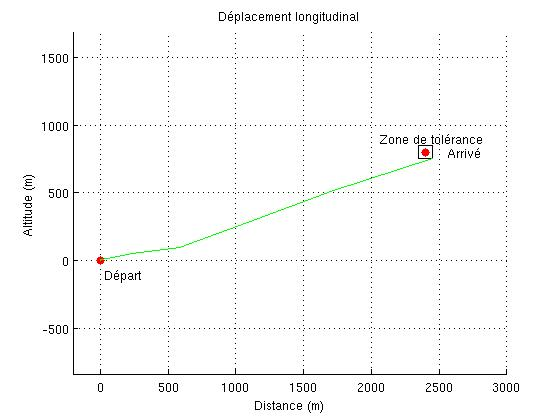
\includegraphics[scale=0.54]{images/resultatCplex1.jpg}
	\caption{Planification de trajectoire sur un monde vide}
	\label{fig:resultatCplex1}
\end{figure}

Ces résultats montrent que notre modélisation d'un problème de planification en CSP fonctionne, nous arrivons à déterminer une séquence de commandes permettant la validation de l'objectif.

Néanmoins plusieurs problèmes persistent, l'ajout d'obstacles modifie grandement le temps de calcul du solveur, la variation du temps de la mission également. Dans le tableau suivant sont représentés différentes configurations : 
\begin{center}
\begin{tabular}{|c|c|c|c|c|}
	\hline stepMax & 11 & 13 & 12 & 12 \\ 
	\hline nombres d'obstacles & 0 & 0 & 0 & 1 \\ 
	\hline altitude objectif (m) & 800 & 800 & 800 & 800 \\ 
	\hline distance objectif (m) & 2400 & 2400 & 5875 & 5875 \\ 
	\hline\hline temps de calcul (s) & 1.08 & 325.42 & 1,46 & 7,66 \\ 
	\hline 
\end{tabular} 
\end{center}

Lors de ces tests il nous ait apparu que le temps de calcul été fortement lié au nombre d'itération maximum (lié au temps de la mission) et à la distance à parcourir.

Il est préférable de régler la variable $stepMax$ en fonction de la distance à parcourir, par exemple en prenant en compte la vitesse moyenne, en effet la distance parcourue dépend uniquement du temps de la mission et de la vitesse $Va$. 

La différence de temps de calcul entre les deux premières simulations vient du fait que la distance à parcourir était trop faible vis à vis du temps de la mission, cela implique une vitesse moyenne faible de l'avion (< 100 m/s), alors que la vitesse nominale de notre aéronef est de 235 m/s.
Pour les mêmes raisons, la troisième simulation présente un temps de calcul relativement faible alors que la distance à parcourir est plus grande.

Dans la dernière simulation nous avons placé un obstacle comme présenté dans la figure \ref{fig:resultatCplex2}, alors que cet obstacle ne figurait pas sur la trajectoire initiale (simulation 3), nous pouvons voir que le temps de calcul a déjà augmenté.

En rajoutant d'autres obstacles, et notamment sur la trajectoire initiale, le temps de calcul explose et nous n'arrivons pas à avoir de solution. Nous supposons que cela est du à un problème de convexité de l'espace de recherche mais nous n'avons pas pu vérifier.

\begin{figure}[h]
	\centering	
	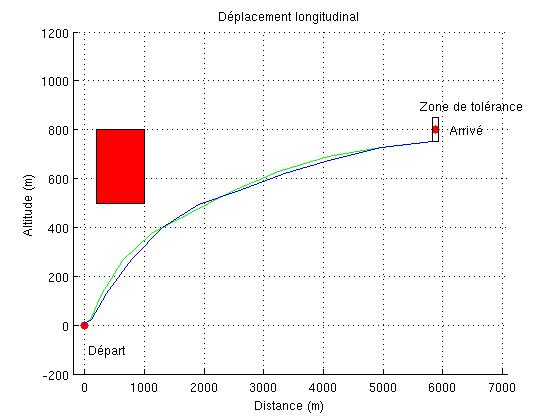
\includegraphics[scale=0.6]{images/resultatCplex2.jpg}
	\caption{Résultat des scénarios 3 (vert) et 4 (bleu)}
	\label{fig:resultatCplex2}
\end{figure}

L'ensemble de ces résultats est encourageant, notre modélisation fonctionne globalement même si des problèmes d'optimisation reste à résoudre. 

\noindent
\shadowbox{\begin{minipage}{\textwidth}
		\textbf{Résumé :} Plusieurs outils ont été testés pour implémenter notre démarche. JaCoP dans un premier temps offre une écriture rapide du problème et des résultats proches de ceux que nous pouvons avoir sur MatLab en terme de précision de calcul sur les espaces d'état. Néanmoins il présente de fortes divergences lors du passage à l'échelle.
		
		Cplex offre un solveur plus performant mais le langage OPL ne nous offre pas assez de possibilité sur l'écriture des variables de types expressions. La librairie JAVA fournie par Cplex semble pouvoir répondre à toute nos attentes, au vue des résultats que nous avons pu avoir, il est nécessaire de se pencher sur l'optimisation de certaines contraintes, ainsi que sur l'utilisation plus avancée du solveur.		
	\end{minipage}}
